\part{Cours Magistral 3 -- Les intégrales}
\section{Introduction}

\begin{center}
\begin{tabular}{l l}

$\int_D f$ &  $f: D\to \mathbb{R}$ \\
&$D$ borné dans $\mathbb{R}^n$
\end{tabular}

\end{center}


\[
\left\{
\begin{array}{l}
D=[a,b]\subset\mathbb{R}\\
D=S\subset\mathbb{R}^2\\
D=V\subset\mathbb{R}^3\\
\end{array}
\right.
\]



\[\int_D 1 = \text{"Volume" de D (longueur de [a,b], aire de S, volume de V)}\]

avec $f\equiv1$
\[ f=\text{densité de matière répartie sur D (par unité de Volume)} \]
\[\int_D f = \text{masse totale répartie dans D = masse de D}\]

Dans ce cours, nous allons voir comment calculer
\begin{itemize}
\item la longueur d'une courbe;
\item l'aire d'une surface
\end{itemize}

\section{Intégrale de ligne d'un champ scalaire}

Voir~\cite{adams2013calculus} p.~875 section~15.3.

Un champ scalaire est une fonction qui associe à chaque point de l'espace ou d'un plan (on parle alors d'un champ scalaire plan) un scalaire. La température dans l'espace à un moment donné est un champ scalaire. On peut également ajouter une composante temporelle (en effet, la température dans l'espace change en fonction du temps). Le champ scalaire sera donc une fonction de $\mathbb{R}^4 \to \mathbb{R} $

\[r=r(t)=x(t)\xunit+ y(t)\yunit+z(t)\zunit = (x(t),y(t),z(t))\]

avec \[a\leq t\leq b\] et où r est le vecteur position d'un point de la courbe C dans le repère ($\xunit,\yunit, \zunit$)

\textbf{Représentation paramétrique de C :}

Droite $d$ scalaire $f(x,y,z)$ donnée $\to \int_C f$
\[a=t_0<t_1<t_2<\dots<t_n=b\]

On va donc calculer les points
\[r_i = r(t_i)\]

Dans chaque segment arbitrairement choisi
\[t_i^*\in[t_{i-1},t_i]\]

\[r_i^*=r(t_i^*)=(x_i^*,y_i^*,z_i^*)\]

Maintenant, nous allons former les sommes de Riemann appelées $S_n$
\[S_n=\sum_{i=1}^nf(x_i^*,y_i^*,z_i^*)\norm{\Delta r_i}\]

Passage à la limite $n\to\infty$; max$\abs{\Delta r_i}\to 0$

\[I=\int_C f = \int_C f (x,y,z)\dif S\]

où $\dif S$ est la longueur d'arc infinitésimale.

\begin{mytheo}
Si (condition suffisante) C est de classe $C^1$ et est continue sur C, alors $\int_C f$ existe\\
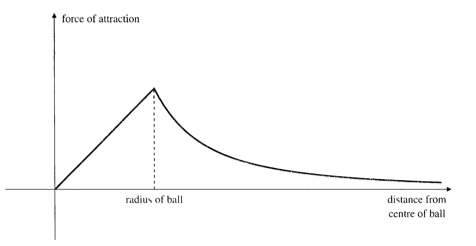
\includegraphics[scale=0.5]{exemple1.png}\\
La fonction n'est pas de classe $C^1$
\end{mytheo}

\begin{myrem}

$f\equiv1$
\[\int_C 1 = \int_C \dif S = \text{longueur de la courbe entre le point de départ et le point d'arrivée}\]
\end{myrem}

\begin{myrem}
Si $f$ est une densité de matière par unité de longueur, alors $\int_C f  = \text{masse totale répartie le long de }C$
\end{myrem}

On reprend la formule
\[S_n=\sum_{i=1}^nf(x_i^*,y_i^*,z_i^*)\norm{\Delta r_i}\]
 et on pose \[\norm{\Delta r_i }=\frac{1}{\Delta t_i}\norm{\Delta r_i} \Delta t_i\]


 \[\lim_{\Delta t_i \to 0} \frac{\Delta r_i}{\Delta t_i} = \frac{\dif r}{\dif t}(t=t_i)\]

\fbox{
\begin{minipage}{10cm}


\textbf{Formule à connaître \# 2 }\\
 \textit{Règle de calcul}
 \[\int_C f = \int_C f (x,y,z)\dif S = \int_a^b f(r(t))\norm{\frac{dr}{dt}} \dif t\]
 $f(r(t))$
 évalué le long de la courbe $f(x(t),y(t),z(t))$
 
 Cette formule sert à calculer l'intégrale d'un champ scalaire sur une ligne.
 \end{minipage}
 }
\\

 Exemple :

 Demi-cercle centré à l'origine de rayon $a$. Le point $(x,y)$ se trouve à une amplitude $t$ par rapport au point $(a,0)$

 \[\int_C y \dif S\]

 \begin{itemize}

 \item
 \[r(t) = (a \cos t ) \xunit + ( a \sin t )\yunit +0k\]
avec $ 0\leq t \leq r $ et $a \cos t =x(t)$ et $a \sin t = y(t)$ et $t$ croissant $(\dif t>0)$

Dès qu'on a choisi une représentation, on a choisi un sens de parcours.
\item
\[\frac{\dif r}{\dif t}=(-a\sin t )\xunit + (a \cos t ) \yunit\]

 où $(-a\sin t ) = \frac{\dif x(t)}{\dif t}(t)$ et $(a\cos t ) = \frac{\dif y(t)}{\dif t}(t)$

\item \[\norm{\frac{\dif r}{\dif t}}=a\]
\item \[I = \int_C y \dif s = \int_0^{\pi} f(r(t))a\dif t\]

$f(r(t))$ est calculé le long de la courbe $= y$ sur la courbe
\[I=\int_0^2 a \sin{t} \, a \dif t = -a^2 \cos t \Big \rvert^\pi_0 =2a^2\]
 \end{itemize}

Nous pouvons choisir une autre représentation paramétrique de la courbe C et nous obtiendrons le même résultat.

\[x^2+y^2 = a^2\]

On choisit $x$ comme paramètre.

Dans le dessin d'un demi-cercle de rayon $a$

\[x \in [-a;a]\]
\[y=\sqrt{a^2-x^2}\]
\[r(t) = (x)\xunit + \sqrt{a^2-x^2} \yunit\]

Quand on va de $-a$ à $a$, on parcourt la courbe mais dans l'autre sens. On a choisi une autre représentation paramétrique. Faire l'exercice à la page 859 et on trouvera le même résultat, c'est-à-dire $2a^2$

On peut donc conclure que

$I=\int_C f \dif S$ ne dépend pas du choix de la représentation paramétrique de C. Et c'est normal parce que pour un problème physique, la masse d'un objet ne peut pas dépendre de la méthode mathématique que l'on utilise pour la calculer.

\section{Intégrale d'un champ scalaire sur une surface}
Voir~\cite{adams2013calculus}, p.~887 section~15.5
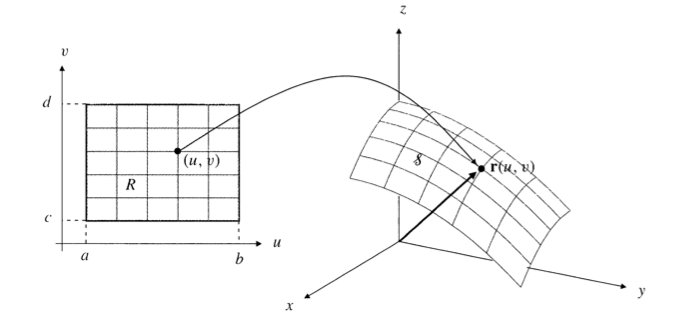
\includegraphics[scale=0.5]{courbe1.png}%p832
\\
Il y a un mapping $r(u,v)$ de $\mathbb{R}$ dans $S$. À partir du quadrillage initial, on obtient des courbes correspondantes.


\[\vec r(u,v)=x(u,v)\xunit +y(u,v)\yunit +z(u,v)\zunit\]

avec $(u,v)\in \mathbb{R}$

On peut considérer que le bord de $R$ est projeté sur les bords de $S$. Mais, ici, on ne demande pas que l'application (le mapping) soit \emph{bijective}.

Exemple : \[r(u,v) = (a \cos u \sin v) \xunit + (a \cos u \sin v) \yunit +(a \cos v) \zunit\]

avec $a \cos u \sin v = x(u,v)$, $(a \cos u \sin v)=y(u,v)$ et $(a \cos v) =z(u,v)$

\[
R=
\left\{
\begin{array}{c}
0\leq u \leq 2 \pi ; 0\leq v\leq \pi /2\\

a = \textbf{cst} > 0
\end{array}
\right\}
\]

C'est une demi-sphère d'équation

\[x^2+y^2+z^2 = a^2\]

Domaine :
$u$ va de $0$ à $2\pi$ et $v$ va de 0 à $\pi /2$

Par le mapping, un point du rectangle du domaine va vers un point de la demi-sphère.

Tous les points sont transformés en \[\vec r (u,\pi/2 ) = (a \cos u  )\xunit + (a \sin u )\yunit \] avec $0\leq u \leq 2 \pi $

\[v=0 \to r(u,0) = 0 \xunit + 0 \yunit + a \zunit\] autrement dit, le point (0,0,a)


Le bord de la demi-sphère n'est défini que par une partie du bord du rectangle (quand $v=\pi/2$ et que $u$ varie de $0$ à $2\pi$).
Il n'y a pas de bijection mais ce n'est pas grave.


\[\int_S f(x,y,z)\dif S\]

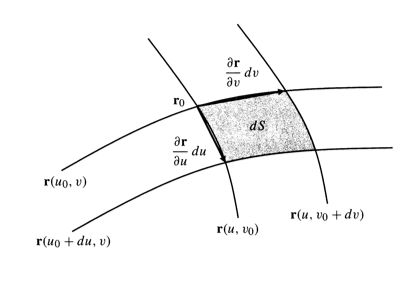
\includegraphics[scale=0.5]{courbe2.png}

On a trouvé ce graphique en partant d'un rectangle où $u$ va de $u_0$ à $u_0 + \dif u$ et $v$ va de $v_0$ à $v_0+\dif v$

Pour déterminer une telle intégrale, nous avons besoin de la somme de Riemann.

\[S_n = \sum_{i=1}^nf(x_i^*,y_i^*,z_i^*) \Delta S_i\]

Dans la formule, $\int_S f(x,y,z)\dif S$,

\[f(x,y,z)=f(r(u,v))\] Mais on ne connait pas la valeur de $dS$

Voir le schéma ci-dessus.

$\frac{\partial \vec r }{\partial u } \text{ et } \frac{\partial \vec r }{\partial v }$ sont évaluées en $(u_0,v_0)$

\[\dif S = \norm{\frac{\partial r }{\partial u } \times \frac{\partial r }{\partial v }} \dif u \dif v\]

La signification géométrique de $ \frac{\partial r }{\partial u } \times \frac{\partial r }{\partial v }$ est le vecteur tangent au point $r_0$.

Il n'y a plus qu'à calculer.

\[\frac{\partial r }{\partial u} =
\left( \frac{\partial x}{\partial u}(u,v)\right)\xunit +
\left( \frac{\partial y}{\partial u}(u,v)\right)\yunit +
\left(\frac{\partial z}{\partial u}(u,v)\right)\zunit
\]


\fbox{
\begin{minipage}{10cm}

\textbf{Formule à connaître \#3}
\[
\frac{\partial (F,G)}{\partial (x, y)} =
\begin{vmatrix}
\frac{\partial F}{\partial x}& \frac{\partial F}{\partial y}\\
\frac{\partial G}{\partial x}& \frac{\partial G}{\partial y}
\end{vmatrix}
=\frac{\partial F}{\partial x} \frac{\partial G}{\partial y}- \frac{\partial F}{\partial y}\frac{\partial G}{\partial x}
\]

\[dS=\sqrt{\left(
\left( \frac{\partial(y,z) }{\partial (u,v)}\right)^2 +
\left( \frac{\partial(z,x) }{\partial (u,v)}\right)^2 +
\left( \frac{\partial(x,y) }{\partial (u,v)}\right)^2
\right)}
\dif u\dif v\]


\[\int_S f = \int _S f(x,y,z) \dif S = \iint_R f(x(u,v),y(u,v),z(u,v)) \dif S\]

Avec cette formule, nous pouvons calculer l'intégrale d'un champ scalaire sur une surface.
\end{minipage}
}

Cas particulier : $f\equiv 1 : \int_S 1 = \int_S \dif S = \text{aire de S}$

\[f \equiv 1 = \int_C 1 = \int_C \dif S = \text{longueur de la courbe}\]


\textbf{Exemple }: Un graphique dont le domaine représente une surface D et dont l'aire représente une surface $S=$ graphe de $g$.


 $g(x,y) : D\subset\mathbb{R}^2 \to \mathbb{R}$ donné


Comment calculer $\int_Sf \dif S$ ? Il faut trouver la représentation paramétrique par exemple
$x=u; y=v; z=g(u,v)$

$\forall (u,v) \in D $


\[\Rightarrow r (u,v) = (u)\xunit+(v)\yunit+(g(u,v))\zunit\]

On peut lancer l'algorithme.

On cherche d'abord tous les déterminants.

\[\frac{\partial (y,z)}{\partial (u,v)} =
\begin{vmatrix}
\frac{\partial y}{\partial u}& \frac{\partial y}{\partial v}\\
\frac{\partial z}{\partial u}& \frac{\partial z}{\partial v}
\end{vmatrix} =
\begin{vmatrix}
0&1\\
\frac{\partial g}{\partial u}&\frac{\partial g}{\partial v}
\end{vmatrix}
= \frac{-\partial g}{\partial u}\]
Un autre,
\[\frac{\partial (z,x)}{\partial (u,v)} = \frac{-\partial g}{\partial v}\]
et le dernier,
\[\frac{\partial (x,y)}{\partial (u,v)} = 1\]

On calcule

\[\int_S f = \iint_D f(x,y,g(x,y)) \dif S = \iint_D f(u,v,g(u,v))\sqrt{1+(\frac{\partial g}{\partial u})^2 +(\frac{\partial g}{\partial V})^2 } \dif u\dif v
\]

avec $f$ évaluée sur la surface.

\section{Intégrale de la composante tangentielle d'un champ de vecteur $F(x,y,z)$ le long d'une courbe $C$}

Voir~\cite{adams2013calculus}, p.~879, section~15.4\\


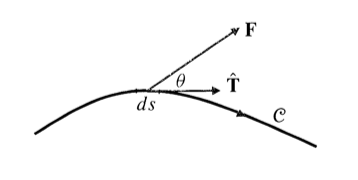
\includegraphics[scale=0.5]{vec1.png}\\

\[\dif W = \vec F\cdot \vec \dif r = F\cdot \hat{T} \dif S\]
et $\hat{T}$ est la tangente unitaire à $C=\frac{\dif r}{\dif t}\frac{1}{\norm{\frac{\dif r}{\dif t}}}$. C'est une dérivée partielle.

(Voir~\cite{adams2013calculus} section~11.4 ou la partie du cours donnée par M. Glineur).

\[\dif W = \norm{F} \cos \Theta \dif S\]
On souhaite calculer

\[\int_{A\to B} \dif W = \text{travail total exercé par la force F sur la particule le long de C}\]


\[\vv{F}=F_1 \xunit + F_2 \yunit +F_3 \zunit\]
\[\vv{F} = \vv{F}(x,y,z)\]

On cherche
\[\int_C\vv{F}\cdot \hat T \dif S\]

et $\cdot$ est un produit scalaire. Le résultat est un \emph{scalaire}.

\[= \int_C F\cdot \dif r = \int_C \vv{F}\]

En fait, c'est l'intégrale de la composante tangentielle du vecteur.

$\int_C F\cdot \hat T \dif S$ est une intégrale de type connu. Elle peut être écrite sous la forme $\int_C f \dif S$ où $f=F \cdot \hat{T}$

L'intégrale dans un sens est l'opposé de l'intégrale dans l'autre sens.

\[I^{\ominus} = -I^{\oplus}\]



\fbox{
\begin{minipage}{10cm}
\textbf{Formule à connaître \# 4}
\[r(t)= x(t)\xunit+y(t)\yunit+z(t)\zunit\]
$a\leq t\leq b$

$$\int_C F = \int_C F\cdot \dif r = \int_C ( F \cdot \frac{\dif r}{\dif t}) \dif t $$
\[= \int_a^b \left[F_1( x(t),y(t),z(t)) \frac{\dif x(t)}{\dif t}+
F_2( x(t),y(t),z(t)) \frac{\dif y(t)}{\dif t}+\right.\]
\[\left.
F_3 (x(t),y(t),z(t)) \frac{\dif z(t)}{\dif t}\right]\cdot dt\]

Cette formule nous montre comment calculer l'intégrale d'un champ vectoriel sur une ligne.
\end{minipage}
}
\\
\\
\textbf{Exemple 1} :
Un champ vectoriel qui a pour équation :
\[F(x,y)=(y^2)\xunit+(2xy)\yunit\]

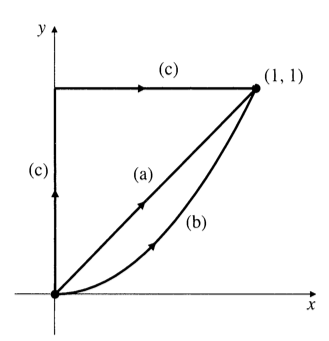
\includegraphics[scale=0.6]{courbe3.png}\\
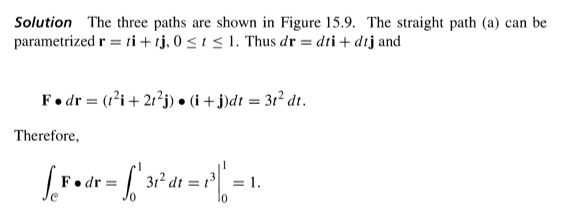
\includegraphics[scale=0.6]{resolu1.png}

Sur les deux autres chemin, on va toujours trouver 1. Il y a beaucoup de chance que cette force soit conservative mais c'est possible que non. Pour en être sur, il faudrait calculer par tous les chemins possibles et voir si on a toujours le même résultat. Pour ça, on applique le Théorème de Poincaré (cf. CM4). D'un point de vue mathématique, on se demande si c'est un champ de vecteur conservatif. Le Théorème de Poincaré nous permettra de le déterminer.

\begin{mytheo}[Théorème de Poincaré]
Voir plus tard.
\end{mytheo}
\textbf{Exemple 2 }: \[F=y\xunit-x\yunit\]

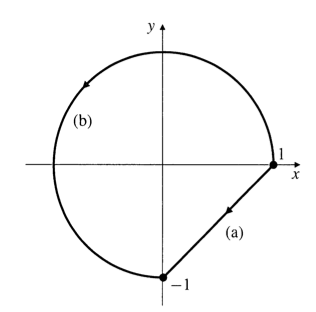
\includegraphics[scale=0.7]{resolu2.png}
\[\int_C F \cdot \dif r\]
\[
\left\{
\begin{array}{l}
I(a)=1\\
I(b)=-3\pi/2
\end{array}
\right.
\]

Avec les deux chemins, on ne trouve pas le même résultat. F n'est donc évidemment pas conservative.
